\section{Approach}
\label{sec:approach}

First we give a short outline of our approach and then
  we provide a more detailed description of the individual steps.

\subsection{Outline of the approach}

We start by assuming that we are given an identity relation $\approx$.
We will then reinterpret this relation as an indiscernibility relation
  relative to different sets of predicates.
Pairs that have the same indiscernibility predicates
  are simi-discernible, i.e.: they discern resources
  based on the same criteria.
Simi-discernibility is an equivalence relation
  which partitions all pairs and thus also the identity relation $\approx$.
The members of the indiscernibility partition
  have a certain overlap with the original identity relation.
The overlap between an indiscernibility subset and the identity relation
  is called an \emph{identity subrelation}.
Each identity subrelation is characterized in terms of predicates
  from the domain vocabulary.
Different forms of identity can therefore be distinguished
  and meaningfully described.
Based on whether there is a complete or a partial overlap
  between the simi-discernible partition members and
  the identity subrelations,
  these partition members belong either to the lower ($\lowerapprox$)
  or to the higher approximation ($\higherapprox$) of $\approx$.
Besides setting a lower and a higher bound to the identity relation,
  we can also calculate the quality of the identity relation
  and the precision of each identity subrelation.

\subsection{Preliminaries}
\label{sec:preliminaries}

RDF terms that occur in the predicate position of an RDF triple are
  \textbf{RDF predicate terms}.
An example from the IIMB dataset is \verb|IIMBTBOX:spoken_in|.
This is not the same as the terms that \emph{can} occur
  in the predicate position of a triple,
  since any URI can occur in this position,
  but some URIs denote non-propery resources.

The interpretation of an RDF predicate term is an \textbf{RDF property},
  which is an RDF resource.

The extension of an RDF property is a \textbf{binary FOL relation},
  i.e. a subset of the cartesian product of the domain
  \footnote{In RDF the domain is the set of RDF resources.}.

A \textbf{FOL property} is a subset of the domain.

The correlate of a FOL property in RDF is a pair
  consisting of a predicate and an object term (in that order).
We call this syntactic construct a \textbf{$PO$-sequence}.
The extension of the interpretation of a $PO$-seq is
  $Ext(I(p))(I(o))$, which is a set of RDF resources.

\begin{itemize}
\item RDF `graph' $G$.
\item RDF subject terms $S_G$.
\item RDF property terms $P_G$.
\item RDF object terms $O_G$.
\item The set of blank nodes $\mathcal{B}$ (definition \ref{def:blank_node}).
\item The set of plain literals $\mathcal{LP}$ (definition \ref{def:plain_literal}).
\item The set of typed literals $\mathcal{LT}$ (definition \ref{def:typed_literal}).
\item The canonical mapping for a datatype $d$, $c_d : LEX_d \rightarrow V_d$.
\item An interpretation function $\mathcal{I}$.
\item Canonical projecting map
  \[
    \pi : (\mathcal{B} \union \mathcal{I})
  \rightarrow
    (\mathcal{B} \union \mathcal{I})/\sim
  \].
\item $\equivset{p}$ is the equivalence class for $p$ under $\approx$.
\end{itemize}

In the following we consider an arbitrary,
  materialized RDF graph $G$ and an identity relation $\approx$ over
  the resources that occur in $G$.
The subject terms of $G$ are denoted by $S_G$, the predicate terms by $P_G$
  and the object terms by $O_G$.


\subsection{Shared properties and indiscernibility}
\label{sec:indiscernibility}

When we look at the triples that constitute a set of identity relations,
  we see that all links look the same.
But when we take the triples in which the subject and object terms occur
  into account, we see that within the identity relation there may be
  different subrelations that we can identify in terms of the predicates
  that occur in the schema.

For instance, in the IIMB dataset there are some identical resources that
  share the property \verb|IIMBTBOX:spoken_in|, while other pairs share
  the property \verb|IIMBTBOX:form_of_government|.
The set of pairs of resources that are spoken in the same language may even
  be disjoint from the set of pairs of resources that have the same
  form of government.

Note that we are not only interested in the properties that resources share
  with one other (e.g., where they are spoken, or which form of government
  they have), but we are also interested in resource pairs that share
  the same sharing properties.
We can thus identify subsets of an identity relation based on differences
  in the sets of predicate path maps relative to which they take resources
  to be \emph{indiscernible} from one another.

In the example above, one subset of the identity relation does not discern
  resources that are spoken in the same language, whereas another subset
  of the identity relation does not discern resources that have the same
  form of government.

We say that two resources are indiscernible with respect to
  a set of predicate path maps $P \subset P_G^n$
  in case they share the same properties denoted by those ppms
  (def. \ref{def:resource_indiscernability}).\footnote{
    $P$ must be closed under the identity relation, i.e.,
    \begin{equation*}
      cl_{\sim}(P) = \bigcup_{\tuple{\range{p_1}{p_n}} \in P}\nolimits (
        [p_1]_{\sim} \times \ldots \times [p_n]_{\sim}
      )
    \end{equation*}}
We say that two resource pairs are indiscernible
  in case both pairs are indiscernible for the same
  $P^* \subseteq \mathcal{P}(P_G^n)$
  (def. \ref{pair indiscernibility}).\footnote{
    In order to assertain that $f_p(x)$ and $f_p(y)$ denote
      the same set of resources, identity does not suffice.
      $\approx$ gives a special treatment for blank nodes and
      typed literals (skipped here for brevity).
  }

\small
\begin{definition}[Indiscernibility]
\begin{align}
\label{def:resource_indiscernability}
\mathit{IND}(P) \,=\,
  \setdef{
    \pair{x}{y} \in S_G^2
  }{
    \forall_{p \in cl_{\sim}(P)} f_p(x) \approx f_p(y)
  }
\\
\label{pair indiscernibility}
\mathit{IND}(P^*) \,=\,
  \setdef{
    \pair{\pair{x_1}{y_1}}{\pair{x_2}{y_2}} \in (S_G^2)^2
  }{\\
    \forall_{P \in P^*}
        \pair{x_1}{y_1} \in \mathit{IND}(P)
      \leftrightarrow 
        \pair{x_2}{y_2} \in \mathit{IND}(P)
  }\nonumber
\end{align}
\end{definition}
\normalsize

\noindent As explained above, for a given set of identity pairs there
  may be multiple pairs that have the same shared properties.
These sets of predicates that are shared across resource pairs are
  considered to give a description of a specific subrelation of
  the identity relation.

According to the standard definition,
  identical resources are indiscernible with respect to all properties.
We take a given set of identity pairs and partition it into subsets which
  we can describe as being $cl_{\sim}(P)$-indiscernible,
  for $P \subseteq P_G^n$.

Fig. 1 shows an example
  of a discernibility partitioning for a given identity relation.

\begin{comment}
\begin{figure*}
\label{fig:iimb_example}
\centering
\includegraphics[width=\textwidth]{iimb_approximation_example_crop}
\caption{
  An example of a discernibility partition for an identity relation
    consisting of 365 pairs applied to the fourth IIMB linkset.
  Each node is annotated with the set of predicates $P$ for which
    its pairs are $P$-indiscernible.
  The number of identity pairs within each partition set
    is displayed to the right of the predicate set label.
  Partition sets that contain no identity pair are not show.
  The number that occurs to the left of the predicate label in each node
    indicates how may pairs in that node are identity pairs.
  The lower approximation consists of the nodes with a solid border,
    indicating that they contain only identity pairs.
  The higher approximation consists of all displayed nodes.}
\end{figure*}
\end{comment}

\subsection{Approximation}
\label{sec:approximation}

In the previous section we partitioned a given identity relation $\sim$
  into subrelations that can be distinguished in terms of schema predicates
  (or $n$-depth paths of those predicates).
In this section we create an approximation of the identity relation.
This approximation will allow us to
  (1) give suggestions about which pairs to in/exclude from
      the identity relation, and
  (2) give an indicator for the quality of the identity relation.

For the approximation of the identity relation we use
  rough set theory \cite{pawlak_1991} to represent an approximation of
  a given identity relation $\sim$.
The domain for our rough set approach is the Cartesian product of $S_G$.
The set of predicates is the powerset of $P_G$.
%\footnote{
%  Relations are called `attributes' in rough set theory.
%  They are functions that map to an arbitrary set of value labels.
%  We only consider functions that map from binary input into
%    the set of Boolean truth values, and therefore use the term
%    `predicates' to denote these functions.
%}
%This means that we have a big number of primitives to work with
%  (quadratic in the number of constants;
%   exponential in the number of relations).

For an arbitrary binary relation $\sim$ we can define
  a higher (def. \ref{def:higher_approximation}) and
  a lower (def. \ref{def:lower_approximation}) approximation
  of that relation.
In definitions \ref{def:higher_approximation} and
  \ref{def:lower_approximation},
  $\mathbb{R}$ characterizes a similarity relation between resource pairs.
The intuition behind these definitions is that non-$\sim$-pairs
  that are similar to $\sim$-pairs should be in the higher approximation,
  whereas no $\sim$-pair that has a similar non-$\sim$-pair should be
  in the lower approximation.

\small
\begin{definition}[Higher \& lower approximation]
\begin{align}
\label{def:higher_approximation}
x \overline{\sim} y \, & \iff & \,
  \exists u,v (\pair{u}{v} \mathbb{R} \pair{x}{y} \,\land\, u \sim v)
\\
\label{def:lower_approximation}
x \underline{\sim} y \, & \iff & \,
  \forall u,v (\pair{u}{v} \mathbb{R} \pair{x}{y} \,\rightarrow\, u \sim v)
\end{align}
\end{definition}
\normalsize 

\begin{comment}
\small
\begin{definition}[Higher \& lower approximation]
\label{def:higher_lower_approximation}
\begin{align}
  y \in [x]_H
\,\iff\,\\
  \exists u (
      \card{[u]_{\sim}}>1
    \,\land\,
      \mathbb{P}([u]_{\sim})=\mathbb{P}(\set{x,y})
  )\nonumber
\\
  y \in [x]_L
\,\iff\,
  \forall S \subseteq D (\\
      (\card{S}>1 \,\land\, \mathbb{P}(S) = \mathbb{P}(\set{x,y}))
    \,\rightarrow\,
      \exists s \in D (S=[s]_{\sim})
  )\nonumber
\end{align}
\end{definition}
\normalsize
\end{comment}

\noindent Since we want to stay close to the traditional notion of identity,
  defined in terms of indiscernibility,
  we choose $\mathit{IND}(\mathcal{P}(P_G^n))$ as our similarity relation.

Figure 1 shows an example of the lower and higher
  approximations for a linkset.
Since in this figure a partition is only drawn when there is at least one
  identity pair that is indiscernible with respect to some set of
  predicates, the higher approximation amounts to the entire figure.
The lower approximation only consists of those partition sets that contain
  at least one identity pair, and that contain no non-identity pair.

\subsection{Quality}
\label{sec:quality}

Given the rough set representation $\pair{\underline{\sim}}{\overline{\sim}}$
  of identity relation $\sim$, we can calculate the accuracy of this
  approximation with equation \ref{eq:accuracy}.

\small
\begin{equation}
\label{eq:accuracy}
  \alpha(\sim)
\,=\,
  \card{\underline{\sim}} / {\card{\overline{\sim}}}
  %\dfrac{\card{\underline{\sim}}}{\card{\overline{\sim}}}
\end{equation}
\normalsize

The intuition behind the usefulness of equation \ref{eq:accuracy}
  is that the crispness of a set should be proportional to the quality
  of the identity relation on which it is based.
Since a consistently applied identity relation has relatively many
  partition sets that contain either
  no identity pairs (small value for $\overline{\sim}$) or
  only identity pairs (big value for $\underline{\sim}$),
  a more consistent identity relation has a higher accuracy.

Now that we have a formal metric for identity relation quality,
  we can define the characteristics of an ideal identity relation.
Traditionally the ideal identity relation ensures indiscernibility
  for all expressible properties in the language
  (the principle of the indiscernibility of identicals).
According to this traditional view an identity relation becomes of
  higher quality by considering more predicates (or ppms)
  according to which two resources are not allowed to be discernible.
We give a different quality criterion.

We observe that for a given equivalence relation $\sim$
  defined over a domain of resources $S_G$ we can define the notion of
  full discernibility:

\small
\begin{definition}[Discernible model]
\label{def:fully_discernible}
\begin{align}
& \text{A domain $S_G$ is fully discernible w.r.t. a binary relation $\sim$ iff}
\nonumber
\\
 & \forall x,y \in S_G (
    [x]_{\sim}=[y]_{\sim}
  \,\lor\,\,
    \mathbb{P}([x]_{\sim}) \neq \mathbb{P}([y]_{\sim})
  )
\end{align}
\end{definition}
\normalsize

\noindent From this definition it is clear that a domain of discourse
  is fully discernable just in case there exists a binary relation $\sim$
  such that \mbox{$\alpha(\sim) = 1.0$}.


\subsection{Example}

\begin{figure*}
\label{fig:ihierarchy}
\centering
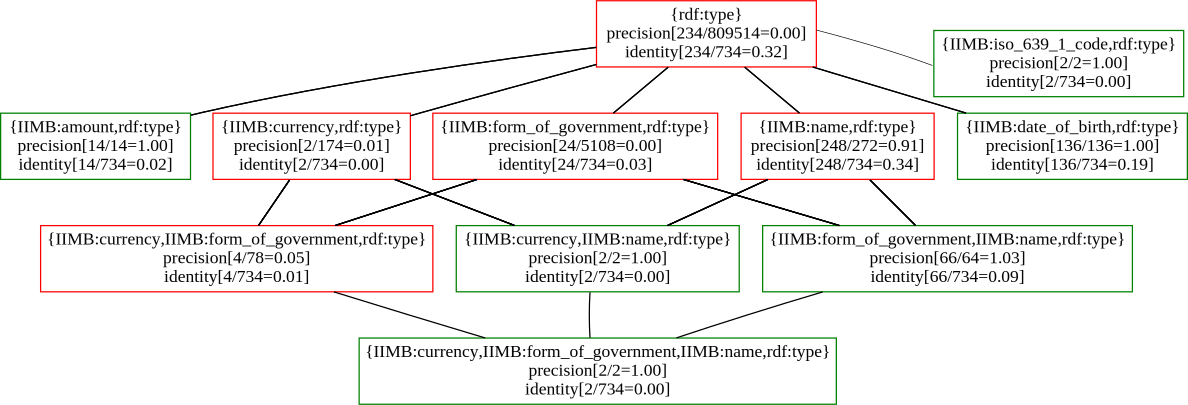
\includegraphics[width=\textwidth]{./img/iimb_16_2}
\caption{
  Example of the identity subrelations for a given dataset (IIMB).
  Each box represents such a subrelation.
  The lower and higher approximation are colored in green and red
    respectively.
  Each box shows the shared predicate terms in curly braces.
  The precision is calculated as
    the number of identity pairs in the subrelation
  divided by
    the number of pairs in the subrelation.
  The identity figure indicates the number of identity pairs in each box,
    divided by the number of identity pairs overall.
}
\end{figure*}

Our approach allows the subrelation hierarchy of a given identity relation
  to be calculated.
Figure \ref{fig:ihierarchy} shows an example of the lower and higher
  approximations for a data- and linkset combination of the IIMB database.
Each rectangular box represents an identity subrelation.
Since in this figure a partition is only drawn when there is at least one
  identity pair that is indiscernible with respect to some set of
  predicates, the higher approximation amounts to the entire figure.
The lower approximation only consists of those partition sets that contain
  at least one identity pair, and that contain no non-identity pair;
  these are distinguished by green borders.

